\documentclass[11pt,a4paper]{article}

\usepackage[utf8]{inputenc}
\usepackage[T1]{fontenc}
\usepackage[english]{babel}
\usepackage{amsmath,amssymb}
\usepackage{booktabs}
\usepackage{graphicx}
\usepackage{siunitx}
\usepackage[hidelinks]{hyperref}
\usepackage{natbib}
\usepackage{geometry}
\geometry{margin=2.5cm}
\usepackage{flafter}   % a float never appears before the text that defines it
% Allow large floats on text pages, so that a tall figure does not get a page
% of its own with most of it left blank.
\renewcommand{\topfraction}{0.85}
\renewcommand{\bottomfraction}{0.5}
\renewcommand{\textfraction}{0.12}
\renewcommand{\floatpagefraction}{0.8}

% ---------------------------------------------------------------------------
% Shared macros — see _research/conventions.md. Do not redefine in sections.
% ---------------------------------------------------------------------------
\newcommand{\SUS}{\ensuremath{\mathrm{SUS}}}
\newcommand{\SEN}{\ensuremath{\mathrm{SEN}}}
\newcommand{\QUANT}{\ensuremath{\mathrm{QUANT}}}
\newcommand{\HEDGE}{\ensuremath{\mathrm{HEDGE}}}
\newcommand{\BREADTH}{\ensuremath{\mathrm{BREADTH}}}
\newcommand{\ESGSI}{\ensuremath{\mathrm{ESGSI}}}
\newcommand{\ESGSIext}{\ensuremath{\mathrm{ESGSI}^{\mathrm{ext}}}}
\newcommand{\Z}{\ensuremath{Z}}
% La etiqueta de especificación va como SUPERÍNDICE para dejar libre el
% subíndice, que §6 necesita para el índice de documento (\susdens_d).
% Con la etiqueta en el subíndice, \susdens_d daba «Double subscript».
\newcommand{\susdens}{\ensuremath{\SUS^{\mathrm{dens}}}}
\newcommand{\sustfidf}{\ensuremath{\SUS^{\mathrm{tfidf}\text{-}\ell}}}
\newcommand{\suslag}{\ensuremath{\SUS^{\mathrm{tfidf}\text{-}L2}}}

\title{Tone Relative to Substance in European ESG Disclosure:\\
A Continuous Corpus-Relative Score, 2018--2024}
\author{}
\date{}

\begin{document}
\maketitle

% ===========================================================================
% PLACEHOLDERS — deliberately not drafted. A human author writes these.
% ===========================================================================
% \input{sections/P1_abstract}
% \input{sections/P2_introduction}
% \input{sections/P3_literature}

% ===========================================================================
% TECHNICAL SECTIONS
% ===========================================================================
\section{Scope and contribution}
\label{sec:scope}

Investors, lenders and supervisors read the ESG sections of
corporate reports, and a recurring concern is that positive language may run
ahead of the content that supports it. This paper measures that relation
directly in the text: how the tone of a report's ESG disclosure stands relative
to the substance of that disclosure. Tone is the polarity of the ESG text under
the finance dictionary of \citet{loughran2011}; substance is the density, in
the same text, of mentions of a documented ESG vocabulary (\S\ref{sec:method}).
We compute the measure for 343 reports of 49 listed firms from seven euro-area
countries, one report per firm and year over 2018--2024 (\S\ref{sec:data}), a
window in which European sustainability reporting moved from largely voluntary
to substantially prescribed.

The measure is a continuous score, and it is relative to the corpus. Each
component is standardised over the 343 reports, so a value locates a report
within this corpus and has no meaning outside it; its sign says only whether
the report lies above or below the corpus mean (\S\ref{sec:method-choices}).
The idea behind the score, positive language in excess of the substance that
supports it, fixes which direction of the score is of interest. The score
describes disclosure, not conduct.

\paragraph{Two scores.} We follow the architecture of \citet{lagasio2024}:
tone relative to substance, measured as a tone component minus a substance
component, each rescaled across the sample. The main score,
$\ESGSI$~\eqref{eq:esgsi}, keeps that architecture and adapts its components
to our corpus and question. The second score, the Extended ESGSI
$\ESGSIext$~\eqref{eq:esgsiext}, is the new metric this paper proposes. It adds
quantification on the side of substance and hedging on the side of tone, with
weights that are a choice rather than an estimate; we report how far the score
moves when they change (\S\ref{sec:robustness}).

\paragraph{Adapting the architecture.} \citet{lagasio2024} introduced the index
on a 2023 cross-section of 749 standalone English-language sustainability
reports. Our question is how tone and substance evolve within the same firms
over seven years, and four design choices follow from it.
\begin{itemize}
  \item \emph{Corpus and extraction.} A balanced panel needs a document that
        every firm publishes every year: for all but one of our firms, the
        annual report or the universal registration document. These filings
        embed ESG disclosure in a much larger financial and legal document, so
        we score the extracted ESG passages rather than whole reports
        (\S\ref{sec:method-extraction}).
  \item \emph{Substance as density.} Substance is the number of ESG mentions
        per 100 words of ESG text, an amount that is comparable across reports
        of very different length (\S\ref{sec:method-choices}).
  \item \emph{Finance dictionary.} Tone is measured with the
        Loughran--McDonald dictionary, built for the language of corporate
        filings.
  \item \emph{A continuous score.} Components are standardised as $z$-scores
        and the score is read as a position in the corpus, with no threshold
        (\S\ref{sec:method-choices}).
\end{itemize}
Because corpus, vocabulary and sentiment dictionary all differ, our scores are
not numerically comparable with those of \citet{lagasio2024}, and no such
comparison is attempted.

\paragraph{Roadmap.} \S\ref{sec:data} describes the corpus and
\S\ref{sec:method} the extraction, vocabulary, scores and inference.
\S\ref{sec:results} reports the scores over time, against the confound of
reporting mandates, by firm group and by pillar; \S\ref{sec:robustness} tests
their sensitivity to the choices of the method, and \S\ref{sec:limitations}
states the limitations.

\section{Data}
\label{sec:data}

The corpus consists of 343 reports of 49 listed firms from seven euro-area
countries, one report per firm and year from 2018 to 2024. The panel is
balanced: every firm contributes seven reports and every year 49. Of the 344
files collected, one 2019 report was present twice, as a re-issue with
identical text, and the copy was removed by comparing document contents. For
each firm-year we take one recurring annual document: an annual report
(235 reports), a universal registration document (URD, 101) or, for one firm,
a standalone sustainability report (7). Table~\ref{tab:data-composition} gives
the corpus by country and document type. The document-type mix barely moves
over time (12 URDs in 2018, 14 or 15 in every later year). Every measure is
computed on the ESG zones extracted from each report, not on whole documents
(\S\ref{sec:method-extraction}). Firms enter the paper only through their
country, their industry and anonymous positions.

Each firm carries one supersector of the Industry Classification Benchmark
(ICB), assigned at firm level and not derived from the reports. The 49 firms
fall into 16 supersectors and 10 of the 11 ICB industries: Financials (11
firms), Consumer Discretionary (10), Industrials (9), Consumer Staples (5),
Health Care and Technology (3 each), and Basic Materials, Energy,
Telecommunications and Utilities (2 each); Real Estate is absent.

\begin{table}[htbp]
\centering
\small
\caption{Corpus composition by country and document type. Industries: number
of ICB industries represented among the country's firms. Every firm
contributes one report in each year from 2018 to 2024.}
\label{tab:data-composition}
\begin{tabular}{@{}lrrrrrr@{}}
\toprule
Country & Firms & Industries & Annual report & URD & Sustainability report & Total \\
\midrule
France      & 17 & 7  & 13  & 99  & 7 & 119 \\
Germany     & 14 & 7  & 98  & 0   & 0 & 98  \\
Netherlands & 6  & 5  & 40  & 2   & 0 & 42  \\
Italy       & 5  & 4  & 35  & 0   & 0 & 35  \\
Spain       & 4  & 3  & 28  & 0   & 0 & 28  \\
Finland     & 2  & 2  & 14  & 0   & 0 & 14  \\
Belgium     & 1  & 1  & 7   & 0   & 0 & 7   \\
\midrule
Total       & 49 & 10 & 235 & 101 & 7 & 343 \\
\bottomrule
\end{tabular}
\end{table}

\paragraph{Country and document type.} Document type is almost entirely
determined by country: 99 of the 101 URDs are French and all 98 German reports
are annual reports, which reflects national reporting practice rather than
sampling. Within the pooled panel a country effect and a document-type effect
can be told apart only through 15 documents (13 French annual reports and 2
Dutch URDs), and the seven standalone sustainability reports belong to a
single French firm. We treat this as a property of the design: no
document-type effect on either score is identified, and since type is constant
within 43 of the 49 firms, firm fixed effects absorb nearly all of it
(\S\ref{sec:method-inference}).

\paragraph{Industry.} Industry cuts across countries: every industry has firms
in at least two countries, and France and Germany each span seven of the ten,
so industry contrasts can be drawn within a single country and document regime
(\S\ref{sec:results-groups}). Industry cannot, however, be separated from the
firm: industries hold 2 to 11 firms, industry is constant within each firm and
so absorbed by firm fixed effects, and because the URD filers are 15 French
firms and one Dutch firm, an industry's URD share is essentially its French
share.

\section{Method}
\label{sec:method}

This section defines every quantity used later in the paper: extraction, the
vocabulary, the components and scores, the reasons for three design choices,
and panel inference (\S\ref{sec:method-extraction}--\ref{sec:method-inference}).

\subsection{Extraction of ESG passages}
\label{sec:method-extraction}

The reports of \S\ref{sec:data} are annual reports and universal registration
documents, in which ESG disclosure is embedded in a much larger financial and
legal document. Scored whole, such a document would let financial-statement
bulk and document length dominate every component. We therefore first extract
its ESG passages; every later measure is computed on them alone.

Each PDF is read as text blocks in reading order, and a block becomes a
paragraph only after five filters: blocks entirely within the top or bottom
8\,\% of the page are dropped; short margin blocks that recur, digits aside, on
more than 30\,\% of a document's pages are dropped as running headers or
footers; tabular blocks (a high share of digits in a few lines, or short
lines of which the first lacks terminal punctuation) are dropped unless they
contain a vocabulary match; short all-capital blocks are taken as section
headings, which label the paragraphs that follow instead of entering the text;
and navigation text (tables of contents, GRI and
ESRS correspondence tables, stray page references), recognised by dotted
leaders, trailing page numbers, multi-level section numbers and disclosure
codes, is dropped, because such lists of ESG section names would otherwise
pass the density rule below. Paragraphs are then stripped of web addresses,
rejoined across line-break hyphenation and collapsed to single spaces.

Each paragraph is matched against the vocabulary of \S\ref{sec:method-vocab}
on its unlemmatised text, ignoring case, with spaces and hyphens
interchangeable between the words of a phrase and longer entries matched before
the shorter ones they contain, so that \emph{carbon footprint} counts once. A
paragraph with at least one match per 100 words is retained together with one
paragraph on each side; overlapping or adjacent windows are merged into a
single zone, and zones shorter than 150 characters are discarded. The zones of
a report, in document order, form its extracted text. Across the 343 reports,
extraction kept 66,171 zones holding 28.1 million of the 71.0 million words of
the PDF text layers, 39.6\,\% (per report, median 38.3\,\%, range
7.1--75.6\,\%). The procedure depends only on the PDF and the vocabulary, and
its recall is bounded by the vocabulary: a passage that uses none of its
entries is never selected.

\subsection{ESG vocabulary}
\label{sec:method-vocab}

Candidate entries came from three sources: the disclosure topics and
terminology of reporting frameworks and standards (GRI, SASB, TCFD and the
ESRS), including the names of the frameworks and regulatory regimes under
which firms label their disclosure; the ESG vocabulary of dictionary-based
studies of corporate disclosure; and a structured review of sample reports from
the corpus, in which independent readers listed the ESG terms they found and
independent evaluators judged the pooled list.
\textbf{[Author: identify the reviewers of the candidate lists.]}
A candidate was admitted if its occurrences in the extracted text, read in
context, predominantly carry an ESG sense (a disclosure, target, data point or
policy on an environmental, social or governance matter). Candidates from the
review had in addition to be dispersed across firms, with at least 50
occurrences in the reports of at least 5 of the 49 firms. A polysemous head was
admitted only inside enumerated collocations (\emph{carbon footprint} rather
than \emph{footprint}; the ESG collocations of \emph{social} and \emph{water}),
and a morphological family or a term carrying digits was written as a pattern
(every word beginning \emph{sustainab-} or \emph{recycl-}; CO$_2$e; Scope 1--3;
ISO standard numbers). Each entry belongs to one pillar: environmental (E),
social (S), governance (G), or transversal (TRANS) for umbrella terms and
reporting regimes (\emph{sustainability}, \emph{ESG}, \emph{CSRD}). Entries
whose occurrences concentrate in one industry are designated sectoral; they are
part of the vocabulary, and excluding them is a sensitivity check
(\S\ref{sec:robustness}). Table~\ref{tab:method-vocab} gives the composition.

Terms were admitted after reviewing a sample of their occurrences in context,
and the frequency-weighted precision of the resulting vocabulary is estimated
from those samples, not measured directly on the final extraction, at about
82\,\%. The stability of the scores under perturbations of the vocabulary is
reported in \S\ref{sec:robustness}.

\begin{table}[tbp]
\centering
\small
\caption{Composition of the ESG vocabulary. Terms and collocations are literal
phrases; a collocation stands in for a polysemous head. Sectoral entries cut
across the three type columns. Scoring entries are the distinct lemmatised
terms (patterns act at extraction only); the last column is their share of the
1,047,951 vocabulary occurrences in the extracted text of the 343 reports.}
\label{tab:method-vocab}
\begin{tabular}{@{}lrrrrrrr@{}}
\toprule
 & \multicolumn{5}{c}{All entries} & \multicolumn{2}{c}{Scoring entries} \\
\cmidrule(lr){2-6}\cmidrule(l){7-8}
Pillar & Terms & Colloc. & Patterns & Total & Sectoral & Entries & Occ.\ (\%) \\
\midrule
E (environmental)   & 123 & 29 & 16 & 168 & 14 & 152 & 38.2 \\
S (social)          & 105 & 23 & 11 & 139 & 14 & 127 & 17.6 \\
G (governance)      &  65 & 27 &  3 &  95 &  8 &  90 & 30.0 \\
TRANS (transversal) &  27 &  3 &  2 &  32 &  0 &  30 & 14.2 \\
\midrule
Total               & 320 & 82 & 32 & 434 & 36 & 399 & 100.0 \\
\bottomrule
\end{tabular}
\end{table}

One vocabulary drives both extraction and scoring: all 434 entries select the
passages, and the 402 terms, lemmatised, are what the substance component
counts. Changing the vocabulary therefore changes the text on which every
component is computed, not only the substance count. For scoring, the extracted
text is lowercased, tokenised and lemmatised with a general-purpose English
language model; stopwords (the standard list and 189 corpus-specific words),
punctuation, numerals and tokens shorter than three characters are removed, and
the vocabulary passes through the same processing, so that each entry is
matched in the representation of the text it is counted on. Eleven phrases that
this processing would empty or reduce to a generic word (\emph{well-being},
both of whose words are stopwords; \emph{say on pay} to \emph{pay};
\emph{ISO 14001} to \emph{iso}) are first replaced by single protected tokens,
in text and vocabulary alike. The 402 terms yield $V = 399$ distinct
lemmatised scoring entries.

\subsection{Components and scores}
\label{sec:method-index}

Let $d = 1, \dots, n$ index the $n = 343$ reports and $j = 1, \dots, V$ the
scoring entries. Each report has two representations of its extracted text:
the \emph{lemmatised text} of \S\ref{sec:method-vocab}, with $L_d$ tokens, and
the \emph{raw text}, with case, digits and stopwords intact, with $R_d$
tokens. Let $c_{dj}$ be the number of occurrences of entry $j$ in the
lemmatised text of $d$, counted over word sequences of one to four tokens (the
length of the longest entry). Entries are counted independently, so an
occurrence of a multi-word entry also counts for any shorter entry it contains.

\paragraph{Substance.} $\SUS$ is the density of ESG mentions, the number of
vocabulary occurrences per 100 lemmatised tokens, with uniform term weights:
\[
\SUS_d \;=\; \susdens_d \;=\; 100 \cdot \frac{\sum_{j} c_{dj}}{L_d},
\]
written $\susdens$ where it is compared with the alternatives of
\S\ref{sec:method-choices}. It uses no document frequencies, so a report's
value does not depend on the other reports in the corpus.

\paragraph{Tone.} $\SEN$ is the Loughran--McDonald polarity
\citep{loughran2011} of the lemmatised text,
\[
\SEN_d \;=\; \frac{s^{+}_d - s^{-}_d}{s^{+}_d + s^{-}_d + \varepsilon},
\qquad \varepsilon = 10^{-6},
\]
where $s^{+}_d$ and $s^{-}_d$ count the tokens whose stem is in the
dictionary's positive and negative lists, and $\varepsilon$ only prevents
division by zero. It is a bounded ratio on $[-1, 1]$ that depends on the
balance of positive and negative words, not on how many there are.

\paragraph{Quantification.} $\QUANT$ is the number of pattern matches per raw
token, summed over four families: percentages; numbers of four or more digits
other than years; physical units (tonnes, CO$_2$e, GHG, energy, power and
volume units); and the names of reporting frameworks (GRI, TCFD,
SASB, CSRD, SDG, the taxonomy and others). It is computed on the raw text
because preprocessing removes numerals.

\paragraph{Hedging.} $\HEDGE$ is the share of the words of the raw text
(letter runs, hyphenated compounds kept whole) that belong to the Uncertainty,
Weak Modal, Strong Modal and Constraining lists of the Loughran--McDonald master
dictionary, 495 word forms taken as written. It is computed on the raw text
because the modal verbs (\emph{may}, \emph{might}, \emph{could}, \emph{must},
\emph{will}) are stopwords. Matching is by form, not by sense: the five most
frequent forms (\emph{risk}, \emph{risks}, \emph{will}, \emph{may},
\emph{requirements}) make up 49.4\,\% of all matches, so $\HEDGE$ registers to
a large extent how often a report names risk.

\paragraph{Breadth and pillars.} $\BREADTH_d = \exp\bigl(-\sum_j p_{dj}\ln
p_{dj}\bigr)$, with $p_{dj} = c_{dj} / \sum_k c_{dk}$, is the effective number
of distinct entries a report uses, a Hill number of order one
\citep{hill1973}; it is a diagnostic, not a component of either score. The
pillar density $100 \sum_{j \in p} c_{dj} / L_d$ counts the mentions of
pillar-$p$ entries per 100 lemmatised tokens, and the four pillar densities sum
to $\SUS_d$; for a set of reports, the pillar share pools the mentions of the
set. Both are descriptive and enter neither score.

\paragraph{Scores.} Each component $x$ is rescaled across the corpus by a
$z$-score, $\Z(x)_d = (x_d - \bar{x}) / \sigma_x$, with $\bar x$ the mean and
$\sigma_x$ the population standard deviation over all 343 reports pooled across
the seven years, so that yearly means of a score are comparable. The two
scores are
\begin{align}
\label{eq:esgsi}
\ESGSI_d    &= \Z(\SEN)_d - \Z(\SUS)_d, \\[2pt]
\label{eq:esgsiext}
\ESGSIext_d &= \Z(\SEN)_d - \Z(\SUS)_d - w_q\,\Z(\QUANT)_d + w_h\,\Z(\HEDGE)_d,
\qquad w_q = w_h = 0.5 .
\end{align}
$\ESGSI$~\eqref{eq:esgsi} is the main score of the paper. It keeps the
architecture of \citet{lagasio2024}, tone minus substance with each rescaled
across the sample, with substance measured by density and tone by a
finance-specific dictionary in place of a general-purpose polarity score. The
Extended ESGSI~\eqref{eq:esgsiext} is the new metric this paper proposes. Quantified disclosure is further evidence of
substance, so $\Z(\QUANT)$ is subtracted, on the same side as $\Z(\SUS)$;
hedging qualifies whatever a report asserts, so $\Z(\HEDGE)$ is added, on the
side of tone. The weights give each added component half the weight of an
original one, so that together they weigh as much as one of them and the
tone--substance contrast remains the core of the score. They are a stated
choice, not an estimate, since no external criterion is available to calibrate
them; \S\ref{sec:robustness} reports the scores over a grid of weights.

Both scores are continuous and corpus-relative: each has mean zero by
construction, and its sign says only whether a report lies above or below the
corpus mean of the combination. We compare positions within the corpus:
differences of means, trends, rank correlations and the overlap of the top and
bottom deciles.

\subsection{Why density, \texorpdfstring{$z$}{z}-scores and no threshold}
\label{sec:method-choices}

\citet{lagasio2024} computes substance with a TF-IDF vectoriser
\citep{pedregosa2011} over an author-built keyword list and discloses four of
its settings: two document-frequency bounds, a vocabulary cap and the range of
word sequences. It does not state whether each document's term vector is
scaled to unit Euclidean length (vector normalisation), nor how the per-term
values become a document score. The aggregation is immaterial once scores are
standardised, since a sum and a mean over the vocabulary differ by the factor
$1/V$. Vector normalisation is the vectoriser's default and all four disclosed
settings depart from defaults; inferring, as a reading and not a finding, that
only departures were reported, the closest reading of the antecedent is
$\suslag$ below. We also compute $\sustfidf$, which differs from $\susdens$
only in the idf weights:
\[
\suslag_d = \frac{1}{V}\sum_j \frac{c_{dj}\,\mathrm{idf}_j}
{\lVert \mathbf{c}_d \odot \mathbf{idf} \rVert_2},
\qquad
\sustfidf_d = 100 \cdot \frac{\sum_j c_{dj}\,\mathrm{idf}_j}{L_d},
\]
where $\mathrm{idf}_j = \ln[(1+n)/(1+\mathit{df}_j)] + 1$ and $\mathit{df}_j$
is the number of reports containing entry $j$.

A term vector and any positive multiple of it have the same unit vector, so
$\suslag$ keeps the mix of terms and discards their amount, a property suited
to retrieval \citep{sparckjones1972,manning2008} but not to a score that sets
tone against the amount of substance behind it. Panel~A of
Table~\ref{tab:method-choices} shows this on the report at the median of
$\susdens$: multiplying its ESG counts by up to 20 raises its density from 6.78
to 33.79 and leaves $\suslag$ unchanged, and diluting it with 152,378 non-ESG
tokens divides its density by 3.5 and leaves $\suslag$ identical. What remains
after vector normalisation is dispersion over terms: the sum of a non-negative
unit vector lies between 1 and $\sqrt{V}$ and grows as mentions spread over more
entries. On our corpus $\suslag$ correlates 0.955 with $\BREADTH$ and 0.405
with $\susdens$; under vector normalisation, the substance component measures
topical breadth, not the amount of disclosure.

\begin{table}[tbp]
\centering
\small
\caption{Why density. Panel~A: a synthetic document written out from the ESG
counts of the report at the median of $\susdens$, with every count multiplied
by $k$, and the real report with 152,378 non-ESG tokens appended; all 343
reports re-vectorised in every run; $\suslag$ relative to the first row of each
block (maximum absolute deviation $3.5\times10^{-18}$). Panel~B: Pearson
correlation with $\QUANT$ ($n = 343$, 49 firms); disjoint bases remove from the
vocabulary the 17 entries also matched by a $\QUANT$ pattern (399 to 382
entries) and restrict $\QUANT$ to percentages and large numbers; 95\,\%
percentile intervals from 9,999 bootstrap samples of firms, each with its
seven reports.}
\label{tab:method-choices}
\begin{tabular}{@{}lrrrr@{}}
\toprule
\multicolumn{5}{@{}l}{\emph{A. Amount of ESG content and the substance specifications}} \\
 & Tokens & ESG mentions & $\susdens$ & $\suslag$ (rel.) \\
\midrule
Amplified, $k = 1$  &  60,951 &  4,131 &  6.78 & 1.000000 \\
Amplified, $k = 2$  &  70,612 &  8,262 & 11.70 & 1.000000 \\
Amplified, $k = 5$  &  99,595 & 20,655 & 20.74 & 1.000000 \\
Amplified, $k = 20$ & 244,510 & 82,620 & 33.79 & 1.000000 \\
\addlinespace
Real report         &  60,951 &  3,984 &  6.54 & 1.000000 \\
Diluted             & 213,329 &  3,984 &  1.87 & 1.000000 \\
\midrule
\multicolumn{5}{@{}l}{\emph{B. Convergent validity: correlation with $\QUANT$}} \\
 & \multicolumn{2}{c}{Full bases} & \multicolumn{2}{c}{Disjoint bases} \\
\cmidrule(lr){2-3}\cmidrule(l){4-5}
 & $r$ & 95\,\% interval & $r$ & 95\,\% interval \\
\midrule
$\susdens$           & 0.6305 & $[0.523,\ 0.732]$ & 0.3992 & $[0.227,\ 0.539]$ \\
$\sustfidf$          & 0.6392 & $[0.550,\ 0.736]$ & 0.4007 & $[0.256,\ 0.535]$ \\
$\suslag$            & 0.2984 & $[0.041,\ 0.551]$ & 0.1850 & $[-0.072,\ 0.483]$ \\
$\susdens - \suslag$ & 0.3321 & $[0.075,\ 0.589]$ & 0.2142 & $[-0.143,\ 0.519]$ \\
\bottomrule
\end{tabular}
\end{table}

An empirical check needs a yardstick built by other means. $\QUANT$ counts
pattern matches on the raw text, with no vocabulary, vectoriser or document
frequencies, and a report that discloses substance should also quantify it
\citep{campbell1959}. On the full bases (Table~\ref{tab:method-choices},
panel~B) density correlates 0.63 with $\QUANT$ and $\suslag$ 0.30, and the
firm-bootstrap interval of the difference excludes zero. The two instruments
share 17 entries (framework acronyms, the taxonomy family, CO$_2$, GHG, ISO
standards) and read the same zones, so we repeat the test on disjoint bases.
Every correlation falls, by 37--38\,\%, and the ratio between the two
specifications does not (2.16 against 2.11), but the interval of the
difference now includes zero: convergent validity corroborates a density
specification without carrying the choice on its own, which rests on the
invariance above. The two density specifications are not separated by this
test (difference 0.009, interval $[-0.018, 0.044]$ on the full bases); we
adopt $\susdens$ because it estimates nothing on the sample.

The antecedent prints its index as a difference of $z$-scores but states that
the components are min--max rescaled, and its published statistics are
min--max: its mean index, $-0.2179$, is the difference of its component means,
$0.3727 - 0.5906$ \citep[p.~6]{lagasio2024}, whereas a difference of
$z$-scores has mean zero. Both score normalisations are increasing affine maps
and preserve ranks within a component; once two components are differenced,
they differ in how they equalise spreads and where they put zero. On our corpus
ranks barely move (Spearman correlation 0.997 between the $z$-score and
min--max versions of $\ESGSI$), but location does: under min--max the mean of
the score depends on where each component's mass sits within its observed
range ($+0.004$ with $\susdens$, $-0.203$ with $\suslag$, on the same
reports), and a single extreme report can shift it. A $z$-score puts each
component's zero at its corpus mean and measures it in its own standard
deviations, so a score's sign and size describe a position in the corpus and
nothing else. The antecedent also assigns every report to one of two classes by
the sign of its index. We apply no threshold of any kind. Zero is the corpus
mean of the combination, so a cut-off on a difference of standardised
components describes the relative location of two distributions, not the
conduct of a firm, and no external benchmark exists against which a boundary
could be calibrated for these reports (\S\ref{sec:limitations}).

\subsection{Inference on the panel}
\label{sec:method-inference}

Write $d = (i, t)$ for the report of firm $i = 1, \dots, M$ in year $t$, with
$M = 49$ in the balanced panel of \S\ref{sec:data}. Trends are estimated with
firm fixed effects, regressing the firm-demeaned outcome on the firm-demeaned
year; in the balanced panel the slope equals the mean of the firm-level
least-squares slopes. Standard errors are clustered by firm with the usual
small-sample correction, and $t$ statistics are referred to a $t$ distribution
with $M - 1$ degrees of freedom, $M$ being the number of firms in the sample
or subsample. Clustering allows any correlation among a firm's seven reports
but not a shock common to all firms in one year, which with seven years cannot
be clustered on; the slope summarises the yearly means. Because 49 clusters
are few, the fixed-effects slope is also tested with a restricted wild cluster
bootstrap \citep{cameron2008}: under a zero slope the residuals are the
demeaned outcomes, each of $B = 9{,}999$ replications multiplies all residuals
of a firm by one Rademacher weight ($\pm 1$ with equal probability), and the
$p$-value is the share of replications whose cluster-robust $t$ is at least as
large in absolute value as the observed one. Slopes by industry or country
interact the demeaned year with group indicators. Each equals the
mean firm slope of its group, but for a group of $M_k$ firms its clustered
variance rests on $M_k - 1$ free contributions and is too narrow for small
groups, so we read group slopes through the $t$ interval on the $M_k$ firm
slopes ($M_k - 1$ degrees of freedom). Equality across groups is tested with a
Wald test on the clustered variance, anti-conservative when a group has a
single firm. Yearly means carry 95\,\% intervals from a regression on year
indicators, clustered by firm.

\section{Results}
\label{sec:results}

This section asks how tone relative to substance moved over 2018--2024 and why, how much of the
movement reporting mandates could account for, and where firms, industries and countries stand.
$\ESGSI$~\eqref{eq:esgsi} and $\ESGSIext$~\eqref{eq:esgsiext} are in corpus standard deviations,
with trends and intervals estimated as in \S\ref{sec:method-inference}. Industries are ordered by
mean $\ESGSI$ throughout.

\subsection{The yearly series and the trend}
\label{sec:results-time}

Both scores fall in every year of the window: mean $\ESGSI$ from $0.502$ in 2018 to $-0.610$ in
2024, mean $\ESGSIext$ from $0.696$ to $-0.802$ (Table~\ref{tab:results-trend},
Figure~\ref{fig:results-time}a). The within-firm trend is $-0.181$ standard deviations per year
for $\ESGSI$ (95\% interval $[-0.250, -0.111]$) and $-0.260$ for $\ESGSIext$ ($[-0.340, -0.180]$),
and both are significant under clustered and bootstrap inference alike ($p < 10^{-4}$). The yearly
intervals nonetheless overlap widely, so the slope summarises an uneven path rather than a
constant rate. The crossing of zero between 2020 and 2021 is not an event, since both scores
average zero over the window by construction, and the standard errors do not cover a shock common
to all firms in one year (\S\ref{sec:method-inference}).

\begin{figure}[tbp]
\centering
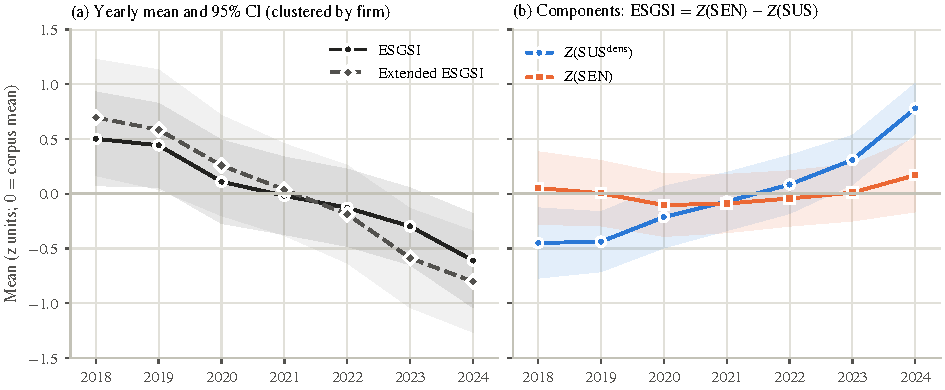
\includegraphics[width=\linewidth]{figures/fig_temporal.pdf}
\caption{(a) Mean $\ESGSI$ and $\ESGSIext$ by year, 49 reports per year, with 95\% intervals
from year indicators and standard errors clustered by firm. (b) The same for $\Z(\susdens)$ and
$\Z(\SEN)$, whose difference is $\ESGSI$ \eqref{eq:esgsi}. All values in corpus standard
deviations; zero is the mean over the 343 reports.}
\label{fig:results-time}
\end{figure}

\begin{table}[tbp]
\centering
\caption{Yearly means and trend regressions; 343 reports of 49 firms, 49 per year. Panel A:
means of the two scores and of their standardised components \eqref{eq:esgsi},
\eqref{eq:esgsiext}; $z$-scores are taken over the pooled corpus (\S\ref{sec:method-index}), so
every row averages zero over the window. Panel B: slope on calendar year with firm fixed effects; standard errors and
95\% intervals clustered by firm ($t_{48}$); $p_{\mathrm{wild}}$ from a wild cluster
bootstrap with 9,999 replications (\S\ref{sec:method-inference}); $R^2_w$ within firm. Component
slopes are in their own units: $\susdens$ in mentions per 100 tokens, $\QUANT$ and $\HEDGE$ in
units of $10^{-4}$, all per year.}
\label{tab:results-trend}
\small
\setlength{\tabcolsep}{4.5pt}
\begin{tabular}{@{}lrrrrrrr@{}}
\toprule
\multicolumn{8}{@{}l}{\textit{A. Yearly means}} \\
 & 2018 & 2019 & 2020 & 2021 & 2022 & 2023 & 2024 \\
\midrule
$\ESGSI$      & $0.502$ & $0.443$ & $0.110$ & $-0.018$ & $-0.128$ & $-0.298$ & $-0.610$ \\
$\ESGSIext$   & $0.696$ & $0.585$ & $0.258$ & $0.038$ & $-0.187$ & $-0.587$ & $-0.802$ \\
$\Z(\SEN)$    & $0.052$ & $0.005$ & $-0.103$ & $-0.090$ & $-0.043$ & $0.011$ & $0.169$ \\
$\Z(\susdens)$ & $-0.450$ & $-0.438$ & $-0.213$ & $-0.072$ & $0.085$ & $0.308$ & $0.779$ \\
$\Z(\QUANT)$  & $-0.402$ & $-0.245$ & $-0.276$ & $-0.073$ & $0.123$ & $0.522$ & $0.351$ \\
$\Z(\HEDGE)$  & $-0.012$ & $0.040$ & $0.019$ & $0.039$ & $0.005$ & $-0.057$ & $-0.034$ \\
\midrule
\multicolumn{8}{@{}l}{\textit{B. Trend}} \\
 & Slope & SE$_{\mathrm{cl}}$ & \multicolumn{2}{c}{95\% interval} & $p_{\mathrm{cl}}$ & $p_{\mathrm{wild}}$ & $R^2_w$ \\
\midrule
$\ESGSI$      & $-0.181$ & $0.035$ & $-0.250$ & $-0.111$ & $3.7\times10^{-6}$ & $<10^{-4}$ & $0.211$ \\
$\ESGSIext$   & $-0.260$ & $0.040$ & $-0.340$ & $-0.180$ & $3.7\times10^{-8}$ & $<10^{-4}$ & $0.295$ \\
$\SEN$        & $0.0020$ & $0.0037$ & $-0.0053$ & $0.0094$ & $0.581$ & $0.577$ & $0.003$ \\
$\susdens$    & $0.366$ & $0.041$ & $0.283$ & $0.449$ & $1.1\times10^{-11}$ & $<10^{-4}$ & $0.364$ \\
$\QUANT$      & $4.7$ & $0.9$ & $2.9$ & $6.5$ & $3.4\times10^{-6}$ & $<10^{-4}$ & $0.206$ \\
$\HEDGE$      & $-0.4$ & $0.8$ & $-1.9$ & $1.2$ & $0.633$ & $0.634$ & $0.002$ \\
\bottomrule
\end{tabular}
\end{table}

What moves is substance. A lower score can mean less positive tone or more substance, and it is
the second (Figure~\ref{fig:results-time}b): $\susdens$ rises in every year, from $5.75$ to $8.05$
mentions per 100 tokens, because mentions per report grow faster ($+205\%$) than the extracted
text that divides them ($+119\%$). Tone does not move: $\SEN$ has no detectable trend ($p =
0.581$), and its yearly means dip in 2020 and rise in 2024, against the decline; a failure to
reject is not a demonstrated null. $\ESGSIext$ falls faster because of quantification: $\QUANT$
rises by about half over the window, though not in every year, while $\HEDGE$ is flat, its
standardised yearly means within $\pm0.06$ of zero. In terms of disclosure practice, the reports
devote a growing part of their ESG text to identifiable ESG content, and put more numbers on it,
without describing it in more positive or more qualified language: the scores fall because ESG
disclosure became denser, not because its tone changed.

The panel is balanced, so the series is not a change in the set of firms or in the country mix,
and the document-type mix barely moves (\S\ref{sec:data}). Within Germany, fourteen firms with
one country and one document type, both slopes are steeper than the pooled ones: $-0.268$ for
$\ESGSI$ ($p = 0.002$; bootstrap $0.003$) and $-0.376$ for $\ESGSIext$ ($p < 0.001$ under both).
A trend of this sign therefore exists where country and document type do not vary, although this
does not show that their mix plays no part in the pooled slope.

\subsection{Regime vocabulary and the mandate confound}
\label{sec:results-mandate}

Over 2018--2024 European sustainability reporting moved from largely voluntary to substantially
prescribed. A firm that adds a taxonomy-alignment table or a standards-referenced sustainability
statement adds ESG vocabulary without necessarily changing anything it does, and $\susdens$
cannot tell the two apart. The vocabulary names regimes that did not exist or were not in force
in 2018, and the transversal pillar that holds them nearly doubles its share of all mentions,
from 10\% to 19\% (\S\ref{sec:results-pillars}).

The purely definitional part can be bounded by deleting entries and rescoring, with the
extraction held fixed. Deleting an explicit list of 22 regime, standard and rating names (3.8\%
of all mentions; deliberately over-inclusive, since several predate the window) leaves an
$\ESGSI$ slope of $-0.149$ ($p < 0.001$), about four fifths of the original, with a rank
correlation of $0.992$ with the full-vocabulary score. Deleting the whole transversal pillar (30
scoring entries holding 21 of the 22 names and 14.2\% of all mentions) leaves $-0.117$ ($p =
0.002$; bootstrap $0.003$), about two thirds, with a rank correlation of $0.973$. $\ESGSIext$ keeps
$-0.228$ and $-0.196$ of its $-0.260$. The trend is not an artefact of counting regime names.

Neither check disposes of the mandate confound. A regime elicits substantive disclosure as well as
its own names (emissions, transition plans, most of the environmental vocabulary) in the words a
firm that had changed its conduct would also use, and the environmental pillar is where the rise
sits (\S\ref{sec:results-pillars}). A mandate is a common time shock, collinear with calendar
year; the balanced panel, the German subsample and the fixed effects remove cross-sectional
composition, not anything that moves with time. Identification would need variation in exposure,
which 49 large issuers, all in scope, do not provide, so the confound is left unresolved. One
consequence belongs to the architecture: since both scores fall when substance rises, a firm that
adds a mandated disclosure moves down the scale for having complied. A user of the scores should
therefore read the decline over this window as denser disclosure, whatever its cause, and not as
evidence that firms became more candid.

\subsection{Firms, industries and countries}
\label{sec:results-groups}

Most of what the scores record is a difference between firms. For $\ESGSI$, 66.7\% of the
variation lies between firm means and 7.2\% between year means, and the correlation between two
reports of the same firm, net of year (the intraclass correlation), is $0.676$ ($\ESGSIext$:
68.5\%, 9.4\%, $0.720$). Positions persist from one year to the next and reshuffle over the window: the Spearman
correlation of firms' $\ESGSI$ between consecutive years averages $0.849$ (range $0.728$ to
$0.915$) but is $0.456$ between 2018 and 2024 ($\ESGSIext$: $0.823$ and $0.393$). The decline is
general but not uniform: 39 of the 49 firm slopes are negative for $\ESGSI$ and 43 for
$\ESGSIext$.

Industry and country are constant within firm, so every comparison between groups rests on 49
firms in cells of one to seventeen (Table~\ref{tab:results-groups}), and every country contrast
is also a document-type contrast (\S\ref{sec:data}).

\begin{table}[tbp]
\centering
\caption{Scores by ICB industry and by country, each ordered by mean $\ESGSI$. Firms: number of
firms, each contributing seven reports. Means are over the group's reports; $\susdens$ in
mentions per 100 tokens. Slope and 95\% interval: group slope and $t$ interval on the group's
firm-level slopes (\S\ref{sec:method-inference}); none for a one-firm group.}
\label{tab:results-groups}
\footnotesize
\setlength{\tabcolsep}{3pt}
\begin{tabular}{@{}lrrrrcrrc@{}}
\toprule
 & & & \multicolumn{3}{c}{$\ESGSI$} & \multicolumn{3}{c}{$\ESGSIext$} \\
\cmidrule(lr){4-6}\cmidrule(l){7-9}
 & Firms & $\susdens$ & Mean & Slope & 95\% interval & Mean & Slope & 95\% interval \\
\midrule
\multicolumn{9}{@{}l}{\textit{Industry (ICB)}} \\
\quad Technology             & 3  & $6.17$ & $1.125$  & $-0.328$ & $[-0.827, 0.171]$ & $1.268$  & $-0.399$ & $[-1.136, 0.338]$ \\
\quad Telecommunications     & 2  & $5.89$ & $0.935$  & $-0.404$ & $[-1.816, 1.007]$ & $0.750$  & $-0.495$ & $[-1.882, 0.892]$ \\
\quad Industrials            & 9  & $6.41$ & $0.297$  & $-0.137$ & $[-0.280, 0.006]$ & $0.200$  & $-0.276$ & $[-0.365, -0.188]$ \\
\quad Consumer Discretionary & 10 & $6.56$ & $0.138$  & $-0.287$ & $[-0.471, -0.103]$ & $0.078$ & $-0.334$ & $[-0.539, -0.128]$ \\
\quad Financials             & 11 & $5.92$ & $0.041$  & $-0.097$ & $[-0.221, 0.027]$ & $0.791$  & $-0.244$ & $[-0.383, -0.104]$ \\
\quad Health Care            & 3  & $6.67$ & $-0.104$ & $0.066$  & $[-0.819, 0.952]$ & $0.013$  & $-0.019$ & $[-0.892, 0.855]$ \\
\quad Basic Materials        & 2  & $7.08$ & $-0.190$ & $-0.437$ & $[-1.236, 0.361]$ & $-0.731$ & $-0.448$ & $[-1.999, 1.103]$ \\
\quad Consumer Staples       & 5  & $7.17$ & $-0.575$ & $-0.239$ & $[-0.374, -0.104]$ & $-0.946$ & $-0.240$ & $[-0.382, -0.098]$ \\
\quad Utilities              & 2  & $9.86$ & $-1.171$ & $0.282$  & $[-0.933, 1.497]$ & $-2.573$ & $0.499$  & $[-3.595, 4.594]$ \\
\quad Energy                 & 2  & $7.33$ & $-1.919$ & $-0.286$ & $[-0.953, 0.381]$ & $-2.642$ & $-0.455$ & $[-0.716, -0.195]$ \\
\midrule
\multicolumn{9}{@{}l}{\textit{Country}} \\
\quad Germany                & 14 & $5.60$ & $1.003$  & $-0.268$ & $[-0.419, -0.116]$ & $1.107$ & $-0.376$ & $[-0.511, -0.241]$ \\
\quad Belgium                & 1  & $6.37$ & $-0.203$ & $-0.372$ & ---                & $-0.043$ & $-0.401$ & --- \\
\quad Finland                & 2  & $6.26$ & $-0.242$ & $-0.123$ & $[-2.287, 2.041]$ & $0.216$  & $-0.399$ & $[-0.565, -0.233]$ \\
\quad France                 & 17 & $6.84$ & $-0.335$ & $-0.182$ & $[-0.296, -0.068]$ & $-0.575$ & $-0.250$ & $[-0.367, -0.132]$ \\
\quad Spain                  & 4  & $8.51$ & $-0.361$ & $-0.055$ & $[-0.336, 0.226]$ & $-0.460$ & $-0.074$ & $[-0.361, 0.214]$ \\
\quad Netherlands            & 6  & $7.04$ & $-0.363$ & $-0.181$ & $[-0.446, 0.085]$ & $-0.031$ & $-0.302$ & $[-0.570, -0.034]$ \\
\quad Italy                  & 5  & $6.65$ & $-0.808$ & $-0.017$ & $[-0.360, 0.325]$ & $-0.817$ & $0.013$  & $[-0.602, 0.628]$ \\
\bottomrule
\end{tabular}
\end{table}

\paragraph{Levels.} Industry means of $\ESGSI$ run from $1.125$ (Technology, three firms) to
$-1.919$ (Energy, two); Utilities has by far the highest $\susdens$ and the second-lowest score.
Both ends rest on two or three firms, dispersion within an industry can exceed the distance
between industries (Financials' firm means span $-1.41$ to $2.09$), and the ordering moves within
the window (Figure~\ref{fig:results-industry}): Basic Materials and Telecommunications go from
well above the corpus mean in 2018 to below it in 2024. $\ESGSIext$ reorders the industries where
quantification and hedging differ most: Financials, with the highest mean $\HEDGE$ and among the
lowest $\QUANT$, moves from $0.041$ to $0.791$, and Utilities, with the highest $\QUANT$, from
$-1.171$ to $-2.573$. Within a single country and document regime, industry does not order firms
reliably: across the $\ESGSI$ firm means it reaches an adjusted $R^2$ of $0.191$ in France (17
firms, seven industries) and of $-0.464$ in Germany (14 firms, seven industries).

Germany stands apart among countries ($1.003$ against $-0.335$ for France), and in each of the
five industries present in both countries the German mean exceeds the French one: the gap
survives holding industry fixed, and so does the document-type contrast it carries. By document
type, annual reports average $0.167$, URDs $-0.263$ and the one firm's sustainability reports
$-1.792$; neither a country nor a document-type effect is identified. At report level, industry
and country each add more to the explained variance of $\ESGSI$ than year does, yet firm identity
still adds $0.301$ of $R^2$ after year, industry, country and document type ($\ESGSIext$:
$0.259$); across the 49 firm means, industry and country together reach an adjusted $R^2$ of
$0.287$ ($\ESGSIext$: $0.421$). Most of the difference between firms is firm-specific: a
report's position says more about its firm's own reporting practice than about the firm's sector
or country.

\begin{figure}[tbp]
\centering
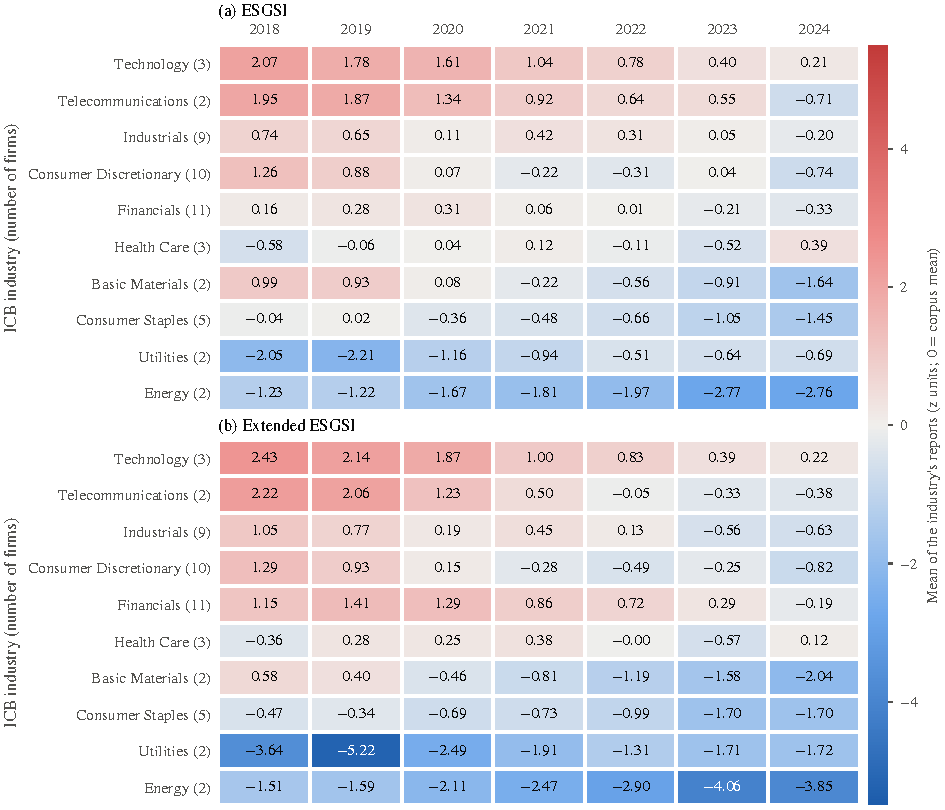
\includegraphics[width=0.76\linewidth]{figures/fig_industry_year.pdf}
\caption{Mean (a) $\ESGSI$ and (b) $\ESGSIext$ by ICB industry and year, in corpus standard
deviations, on a diverging colour scale centred on the corpus mean. Industries are ordered by mean
$\ESGSI$; the number of firms, in parentheses, is also the number of reports averaged in each
cell.}
\label{fig:results-industry}
\end{figure}

\paragraph{Slopes.} Group slopes are read through the intervals on the group's firm-level slopes
(Table~\ref{tab:results-groups}, \S\ref{sec:method-inference}). Utilities shows why: its positive
$\ESGSI$ slope has a clustered interval of $[0.143, 0.421]$ and a firm-slope interval of
$[-0.933, 1.497]$. Read this way, the
$\ESGSI$ decline is distinguishable from zero in Consumer Discretionary (10 firms), Consumer
Staples (5), Germany (14) and France (17); Financials (11) and Industrials (9) have the flattest
declines among the larger industries, with intervals that just include zero. Under $\ESGSIext$,
Financials, Industrials and the Netherlands also decline distinguishably. No group of one to three
firms, including the two industries with a positive slope, supports a statement about its
$\ESGSI$ slope.

\subsection{Pillar composition}
\label{sec:results-pillars}

The rise in mentions is not spread evenly across the pillars of \S\ref{sec:method-vocab}
(Figure~\ref{fig:results-pillars}b). The environmental share of all mentions grows from 32\% in
2018 to 42\% in 2024 and the transversal share from 10\% to 19\%, while governance falls from 39\%
to 23\% and the social share stays between 16\% and 20\%. In density, environmental mentions rise
in every year, from $1.73$ to $3.25$ per 100 tokens, and transversal ones from $0.63$ to $1.52$,
while governance mentions fall from $2.34$ to $1.90$: governance loses ground absolutely, not only
by dilution. The rise in substance is, in other words, environmental and regulatory
(\S\ref{sec:results-mandate}).

\begin{figure}[tbp]
\centering
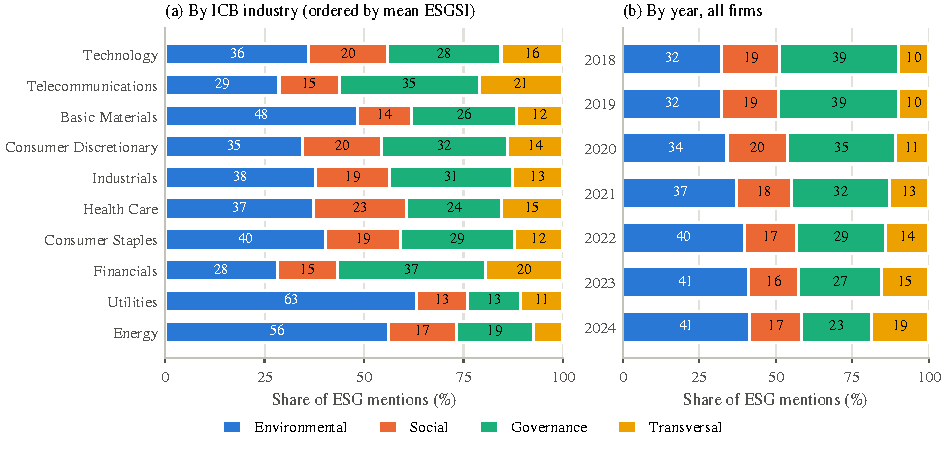
\includegraphics[width=\linewidth]{figures/fig_pillars.pdf}
\caption{Share of all vocabulary mentions falling in each pillar, pooled over the group's
reports, in percent: (a) by ICB industry, ordered by mean $\ESGSI$; (b) by year, all 49 firms.
The unlabelled segment (Energy, transversal) is 8\%.}
\label{fig:results-pillars}
\end{figure}

Across industries the composition follows the business (Figure~\ref{fig:results-pillars}a). The
environmental share runs from 26\% (Telecommunications) to 63\% (Utilities), whose environmental
density of $6.04$ mentions per 100 tokens, against $4.11$ in Energy, the next industry, gives it
the highest $\susdens$ in Table~\ref{tab:results-groups}; Telecommunications and Financials are
the governance-heavy industries (39\% and 38\%). The entries most over-represented in an industry
are its own vocabulary (\emph{hydroelectric} and \emph{smart meter} in Utilities, \emph{oil
spill} and \emph{methane} in Energy), so a firm scores substance partly for describing its
business. The sectoral entries hold 1.0\% of all mentions and at most 2.7\% in any industry
(Consumer Staples), too little to account for the position of Utilities or Energy. Mentions are
concentrated (15 of the 399 scoring entries hold 48.1\% of them); scoring without the sectoral
entries, without each pillar and without the most frequent entry is examined in
\S\ref{sec:robustness}.

\paragraph{Reading the results.} Neither score measures a quantity
(\S\ref{sec:method-choices}): a yearly mean of $-0.610$ is a position within this corpus, and no
level here is comparable with another application of the architecture. What is interpretable is
the ordering within the sample and the direction of change: denser ESG disclosure at unchanged
tone, and firms differing far more than years. None of this is
evidence about conduct: the reporting mandates of the same window could move the scores with
conduct held fixed, and this design cannot exclude them (\S\ref{sec:results-mandate}).

\section{Robustness}
\label{sec:robustness}

A score built on a hand-made vocabulary and chosen weights is useful only if
its conclusions do not hinge on those choices. We vary four of them---the substance specification, the weights of the Extended
ESGSI, the vocabulary and the extraction rule---and compare each variant with a reference score
over the same 343 reports. Every comparison asks three questions. Is the
ranking of reports preserved (Spearman rank correlation $\rho$ with the
reference)? Are the same reports at the extremes (how many of the 34 reports
with the highest, or lowest, reference score remain among the 34 highest, or
lowest, written top/bottom)? And does the trend survive (the within-firm slope
per year, \S\ref{sec:method-inference})?
The reference slopes are $-0.239$ for $\ESGSI$ and $-0.255$ for $\ESGSIext$
(\S\ref{sec:results-time}).

\begin{table}[tbp]
\centering
\small
\setlength{\tabcolsep}{4pt}
\caption{Deletions from the vocabulary under simulated re-extraction
($n = 343$), against the full-vocabulary score as recomputed by the simulation
(slope $-0.239$ for $\ESGSI$ and $-0.255$ for $\ESGSIext$, as for the adopted
scores). Entries: of the 434. Text: share of extracted words
in paragraphs that still qualify (\%). Top/bot: reports of the reference
top/bottom 34 that remain. Slope: within-firm slope per year. Random rows:
medians over 1{,}000 draws (text: mean). With caveat: six frequent entries
admitted although part of their occurrences is navigation text, legal
boilerplate or a non-ESG sense. Late admission: entries that would not pass
the dispersion rule of \S\ref{sec:method-vocab} on the 2018--2019 reports
alone. Late mass: entries with at least three quarters of their occurrences in
2022--2024.}
\label{tab:robustness-summary}
\begin{tabular}{@{}lrrrrrrrr@{}}
\toprule
 & & & \multicolumn{3}{c}{$\ESGSI$} & \multicolumn{3}{c}{$\ESGSIext$} \\
\cmidrule(lr){4-6}\cmidrule(l){7-9}
Deleted & Entries & Text & $\rho$ & Top/bot & Slope & $\rho$ & Top/bot & Slope \\
\midrule
Sectoral entries   & 36  & 99.6 & 0.9983 & 33/32 & $-0.235$ & 0.9988 & 33/33 & $-0.250$ \\
Pillar E           & 168 & 81.1 & 0.8883 & 27/25 & $-0.172$ & 0.9034 & 26/28 & $-0.200$ \\
Pillar S           & 139 & 90.1 & 0.9718 & 31/29 & $-0.222$ & 0.9785 & 32/31 & $-0.243$ \\
Pillar G           & 95  & 68.7 & 0.9048 & 21/28 & $-0.295$ & 0.9461 & 25/28 & $-0.269$ \\
Pillar TRANS       & 32  & 94.8 & 0.9830 & 29/31 & $-0.183$ & 0.9865 & 30/32 & $-0.205$ \\
\emph{Board of directors} & 1 & 93.6 & 0.9936 & 31/31 & $-0.248$ & 0.9906 & 32/33 & $-0.262$ \\
With caveat        & 6   & 95.3 & 0.9902 & 30/31 & $-0.244$ & 0.9927 & 30/33 & $-0.258$ \\
Late admission     & 100 & 99.5 & 0.9950 & 32/32 & $-0.202$ & 0.9955 & 33/33 & $-0.217$ \\
Late mass          & 51  & 99.4 & 0.9879 & 31/31 & $-0.177$ & 0.9891 & 33/33 & $-0.192$ \\
\addlinespace
Random 10\,\%      & 43  & 96.2 & 0.9915 & 32/31 & $-0.234$ & 0.9937 & 32/33 & $-0.249$ \\
Random 20\,\%      & 87  & 92.0 & 0.9804 & 30/30 & $-0.224$ & 0.9849 & 31/32 & $-0.239$ \\
Random 30\,\%      & 130 & 86.8 & 0.9640 & 29/28 & $-0.212$ & 0.9708 & 29/31 & $-0.225$ \\
Random 40\,\%      & 174 & 80.9 & 0.9434 & 27/27 & $-0.199$ & 0.9526 & 28/30 & $-0.211$ \\
Random 50\,\%      & 217 & 73.8 & 0.9145 & 26/25 & $-0.176$ & 0.9245 & 27/28 & $-0.186$ \\
\bottomrule
\end{tabular}
\end{table}

\paragraph{Substance specification.} We recompute $\ESGSI$ with two TF-IDF
versions of substance, in which each entry's count is weighted by how few
reports use it. If the weighted count is divided by the length of the text, as
density is, the ranking is almost unchanged ($\rho = 0.992$; 33/31 of the
extreme deciles kept): how entries are weighted matters little. If instead
each report's vector of weighted counts is scaled to unit length, the ranking
changes markedly ($\rho = 0.626$; 13/19)
and the slope weakens to $-0.198$: how the count is scaled matters much more
(\S\ref{sec:method-choices}).

\paragraph{Weights of the Extended ESGSI.} Over the grid
$w_q, w_h \in \{0, 0.25, 0.5, 0.75, 1\}$ of Eq.~\eqref{eq:esgsiext}, $\rho$
with the score at the default weights is at least 0.826, the minimum being at
$w_q = w_h = 0$, where the score is $\ESGSI$, and at least 0.960 within 0.25
of the default on each axis, where at least 27 of the top and 29 of the
bottom 34 reports remain. The ranking depends mostly on $w_h$; the slope
barely depends on either weight (from $-0.239$ at $w_q = 0$ to $-0.272$ at
$w_q = 1$), is negative in all 25 pairs, and every firm-clustered 95\,\%
interval excludes zero.

\paragraph{Vocabulary.} The vocabulary selects the text as well as scoring it
(\S\ref{sec:method-vocab}), so each deletion of entries is run in two ways:
with the extraction held fixed, so that only the list counted by $\SUS$
changes, and with a simulated re-extraction, in which the extraction rule of
\S\ref{sec:method-extraction} is re-applied without the deleted entries and
all components are recomputed on the paragraphs that still qualify; with the
full vocabulary the simulation reproduces the adopted scores
($\rho = 0.9999$). We delete designed sets of entries and,
1{,}000 times at each size, random sets of 10--50\,\% of the 434 entries, and
read each designed deletion against 1{,}000 random deletions of the same size.
Table~\ref{tab:robustness-summary} gives the re-extraction results for both
scores, and Figure~\ref{fig:robustness-stability} those for $\ESGSI$ in both
modes.

\begin{figure}[tbp]
\centering
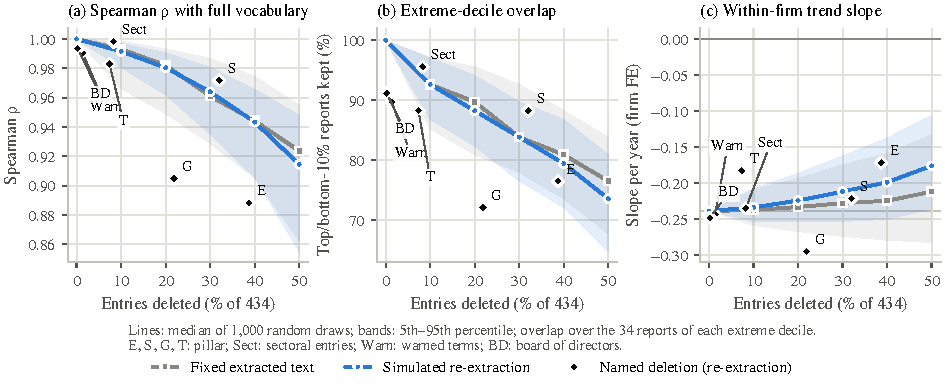
\includegraphics[width=\textwidth]{figures/fig_stability.pdf}
\caption{Stability of $\ESGSI$ under deletion of vocabulary entries
($n = 343$): random deletions in both modes, and the designed deletions of
Table~\ref{tab:robustness-summary} under re-extraction, placed at the share of
the 434 entries they remove (Sect: sectoral entries; T: pillar TRANS; Warn:
entries with a caveat; BD: \emph{board of directors}).
(a) Spearman $\rho$ with the full-vocabulary score. (b) Mean of the top- and
bottom-decile overlaps. (c) Within-firm slope per year; the horizontal line
is the full-vocabulary slope.}
\label{fig:robustness-stability}
\end{figure}

Removing the 36 sectoral entries barely moves either score ($\rho \geq 0.998$
in both modes): they carry about 1\,\% of the vocabulary's matches. The
environmental pillar moves the score most. Without it $\rho = 0.888$, only 25
of the bottom 34 reports remain, and the slope falls to $-0.172$ (SE 0.036,
$p < 0.001$; bootstrap $< 10^{-4}$), still clearly negative. Its $\rho$ is
lower than in 989 of the 1{,}000 random deletions of the same size: the
environmental entries order the reports differently from the rest of the
vocabulary. With pillar G, it is one of the two designed deletions whose
$\rho$ falls below the median for a random half of the vocabulary
(Figure~\ref{fig:robustness-stability}a). With the extraction held fixed its
effect is larger ($\rho = 0.760$, 18 of the bottom 34 kept, slope $-0.135$
with $p < 0.001$), because the paragraphs extracted for
environmental entries stay in the text, unscored, and dilute density. Without the transversal pillar the
slope is $-0.183$; the remaining pillar and entry deletions leave it between $-0.222$
and $-0.295$, the steepest being without pillar G, which also removes nearly a
third of the extracted text. $\ESGSIext$ moves less than $\ESGSI$, in $\rho$,
under every pillar deletion.

Two deletions target the concern that a vocabulary settled on the whole
window favours the language of its last years. Deleting the 100 entries that
would not have passed the dispersion rule on the 2018--2019 reports alone, or
the 51 entries with at least three quarters of their occurrences in 2022--2024
(against 58\,\% of all occurrences), leaves $\rho$ of 0.995 and 0.988 and
slopes of $-0.202$ and $-0.177$: the trend does not rest on entries that only
the later reports qualify.

Under random deletion the ranking degrades smoothly: with half of the entries
removed the median $\rho$ is 0.915 for $\ESGSI$ and 0.925 for $\ESGSIext$,
and 26 of the top and 25 of the bottom 34 reports remain. The slope is the
least stable measure. Under re-extraction its median drifts towards zero as
more is deleted, from $-0.234$ at 10\,\% to $-0.176$ at 50\,\%, because less
of the original text remains; with the extraction held fixed it stays between
$-0.238$ and $-0.212$. Its sign does not change: over the 5{,}000 random
draws the slope of both scores is negative in every draw, in both modes.

\paragraph{Extraction rule.} The same simulation tightens the rule that
selects the text, with the full vocabulary. A threshold of 1.5 or 2 matches
per 100 words, or retaining hot paragraphs without their neighbours, keeps
70--93\,\% of the extracted text and gives $\rho$ between 0.937 and 0.988 and
slopes between $-0.203$ and $-0.260$. A looser rule than the adopted one
cannot be simulated from the extracted text.

\paragraph{An independent text instrument.} As a check of convergent and
discriminant validity \citep{campbell1959}, we apply to the same extracted text,
split into 318{,}258 paragraph-length passages, the open ClimateBERT classifiers
\citep{webersinke2021} with which \citet{bingler2022,bingler2024} build a
cheap-talk index, the share of climate commitments that are not specific. Tone
converges: the classifiers' net climate sentiment correlates with $\Z(\SEN)$ at
$\rho = 0.58$ (95\,\% interval $[0.42, 0.72]$ from resampling firms), within
firms ($r = 0.51$) and between them ($r = 0.62$), and passage by passage (median
within-report $\rho = 0.42$, positive in all but one report). Substance does not
converge with specificity: $\susdens$ tracks the share of climate passages
($\rho = 0.65$) but not the share of specific ones ($\rho = -0.11$; within firms
$r = -0.35$), while $\QUANT$ does, weakly ($\rho = 0.20$). The cheap-talk index
is unrelated to $\ESGSI$ ($\rho = -0.06$, $[-0.27, 0.14]$), to $\ESGSIext$
($0.02$) and to $\HEDGE$ ($0.15$, $[-0.08, 0.35]$), so neither score is a proxy
for cheap talk. In 2024 the classifiers also register a change, but a different
one: fewer passages framed as opportunities and fewer commitments, not more
framed as risks (net sentiment $-0.69$ standard deviations against 2018--2023).
The check shares the text with the scores and covers climate passages only.

\paragraph{Classifiers of the whole text.} Open classifiers that read all of the
extracted text, applied to a random sample of 200 passages per report (67{,}448
passages), point the same way. Sentence-level tone from FinBERT
\citep{huang2023finbert} correlates with $\Z(\SEN)$ at $\rho = 0.77$
($[0.68, 0.84]$; within firms $r = 0.73$, between them $0.86$), in environmental,
social and governance passages alike ($0.66$, $0.69$ and $0.41$), and less with
every other component (with $\Z(\HEDGE)$, $-0.44$). Pillar shares from FinBERT-ESG
and ESGBERT \citep{schimanski2024esgbert} track ours ($\rho = 0.83$ for
governance with both, $0.85$--$0.88$ for the environmental and $0.69$--$0.70$
for the social pillar), and both reproduce the fall of the governance share
(from $0.45$ to $0.29$ and from $0.33$ to $0.21$ of ESG passages between 2018
and 2024). Substance again tracks how much ESG text a report holds (with the
share of passages ESGBERT labels as ESG, $\rho = 0.72$), not how much of it
describes concrete action ($-0.03$ with the share of environmental passages
classified as actions). The classifiers also split the change in tone in 2024
into two parts. The fall of $\Z(\SEN)$ is largest in fragments shorter than 30
words, the rows and labels of the ESRS tables ($-0.47$ standard deviations, and
$-0.10$ without the ESRS topic words of \S\ref{sec:results-time}). Separately,
FinBERT's net tone falls by $0.27$ standard deviations ($[-0.49, -0.06]$), in
environmental and social passages, through fewer positive sentences and not more
negative ones, and by as much without the passages dominated by those words. On
the same passages without those words $\SEN$ does not move ($+0.01$): the
dictionary misses a narrative that became less positive.

Except under unit-length scaling of substance, the ranking of reports is
largely preserved and the trend stays negative; its size depends on the
environmental and transversal vocabulary. These checks bound how far
the scores depend on the choices varied, and the independent classifiers
support the tone component and the pillar composition; they do not validate
the scores as measures of conduct (\S\ref{sec:limitations}).

\section{Limitations}
\label{sec:limitations}

\begin{itemize}
\setlength{\itemsep}{1pt}\setlength{\parskip}{0pt}
\item \emph{No external criterion.} Both scores are positions within this
  corpus and would move if the panel changed. Neither is tested against an
  external criterion (regulatory findings, controversy data, hand-coded
  cases), so no value is evidence about a firm's conduct; the empirical
  checks, convergent validity with $\QUANT$ (\S\ref{sec:method-choices}) and
  with independent classifiers (\S\ref{sec:robustness}), read the same
  extracted text.
  The free external criteria that could be assembled for these firms
  (verified emissions under the EU Emissions Trading System, counts of
  reported controversies, market reactions) showed no detectable association
  and had power only for large effects; a test of consequences would need
  analyst forecasts and commercial controversy data.
\item \emph{A vocabulary built on this corpus.} Candidates, admission
  decisions, pillars and sectoral entries were settled on the 343 reports
  that are scored, with no part held out, and admission rests on the
  judgement of the reviewers of the candidate lists
  \textbf{[Author: identify the reviewers.]}. Its precision is estimated
  rather than measured on the final extraction (\S\ref{sec:method-vocab}),
  and its recall is bounded only indirectly, by the share of the text that
  independent classifiers label as ESG and the extraction misses
  (\S\ref{sec:method-extraction}). The stability of \S\ref{sec:robustness} is
  stability around this fit; it covers deletions of entries, including those
  that qualify only on the later reports, not additions, and the size of the
  trend depends on the environmental and transversal entries.
\item \emph{Country, document type and industry.} Document type is almost
  determined by country (\S\ref{sec:data}), so neither effect is identified
  on its own. Industries hold 2 to 11 firms and supersectors 1 to 7, both
  constant within firm, so group contrasts rest on few firms
  (\S\ref{sec:results-groups}).
\item \emph{Inference.} Standard errors are clustered on 49 firms and checked
  with a wild cluster bootstrap, but they do not cover shocks common to all
  firms in a year, and seven years are too few to cluster on
  (\S\ref{sec:method-inference}).
\item \emph{Mandate.} The content of the mandatory sustainability statement
  became progressively prescribed over the window. The staggered entry of
  taxonomy alignment and of the ESRS gives only weak variation in exposure,
  and it detects no jump (\S\ref{sec:results-mandate}), so the rise in
  substance cannot be split into changed conduct and compliance, and
  compliance itself lowers both scores.
\item \emph{Weights.} The weights of the Extended ESGSI are a choice. Its
  ranking is stable near them but depends on $w_h$ further away, and its
  trend barely depends on either (\S\ref{sec:robustness}).
\item \emph{Dictionaries.} $\SEN$ applies a finance dictionary to
  non-financial narrative, and as a bounded ratio it ignores how many
  sentiment words a text contains. Some negative words of the dictionary
  name ESG topics (\emph{corruption}, \emph{injury}), so a report that covers
  them more reads as more negative, and in 2024 it misses a fall in positive
  narrative tone that two classifiers find (\S\ref{sec:robustness}).
  $\HEDGE$ matches by form, not by sense
  (\S\ref{sec:method-index}).
\end{itemize}

\paragraph{Data and code availability.} The code, the derived data and a
runbook that regenerates every number, table and figure are available in the
project repository. The source reports are public documents published by the
firms.


% \input{sections/P4_discussion}
% \input{sections/P5_conclusion}

\bibliographystyle{elsarticle-harv}
\bibliography{references}

\end{document}
